\pagebreak
\section{The Gain of the Vehicle}\label{app:gainTest}
\textbf{Name: Group 510}\\
\textbf{Date: 13/11 - 2015}

\subsubsection{Purpose}
The purpose of this test is to find the vehicle's gain.

%\subsubsection{Theory}
\subsubsection{Setup}

\begin{figure}[H]
	\centering
	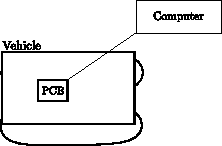
\includegraphics[scale=1.6]{figures/inertiaTestSetupDiagram2.pdf}
	\caption{Setup diagram}
	\label{GainAndTimeTestSetupDiagram}
\end{figure}

\subsubsection{List of Equipment}

\begin{table}[H]
\begin{tabular}{|p{10cm}|p{4cm}|}
\hline%------------------------------------------------------------------------------------
  \textbf{Instrument}                     &  \textbf{Type}       \\
\hline%------------------------------------------------------------------------------------
  Computer                                &  HP 8460P    \\
\hline %-----------------------------------------------------------------------------------
\end{tabular}
\end{table}

\subsubsection{Procedure}

\begin{enumerate}
  \item Disconnect the battery.
  \item Connect the Arduino to the computer.
  \item Upload the test code to the Arduino board using the Arduino IDE  \cite{ArduinoIDE}.
  \item Open a serial terminal via PuTTY \cite{PuTTY}.
  \item Plug in the battery immediately after opening the terminal.
  \item Wait two seconds, then follow the vehicle with the connected computer.
  \item Wait until the vehicle stops before ending the measurements by unplugging the connected computer from the Arduino.
  \item Plot the speed of the vehicle using Matlab.
\end{enumerate}

\subsubsection{Results}
To get as close as possible to the vehicle's exact gain, a test where the vehicle drives at different speed has been set up. In \figref{SpeedStepGainTest} the data from the performed test is illustrated. 

\begin{figure}[H]
  \centering
 	%Trim margins @:   left        bottom       right       top
 	\adjustbox{ trim = {.15\width} {.30\height} {.15\width} {.30\height}, clip }
  {
    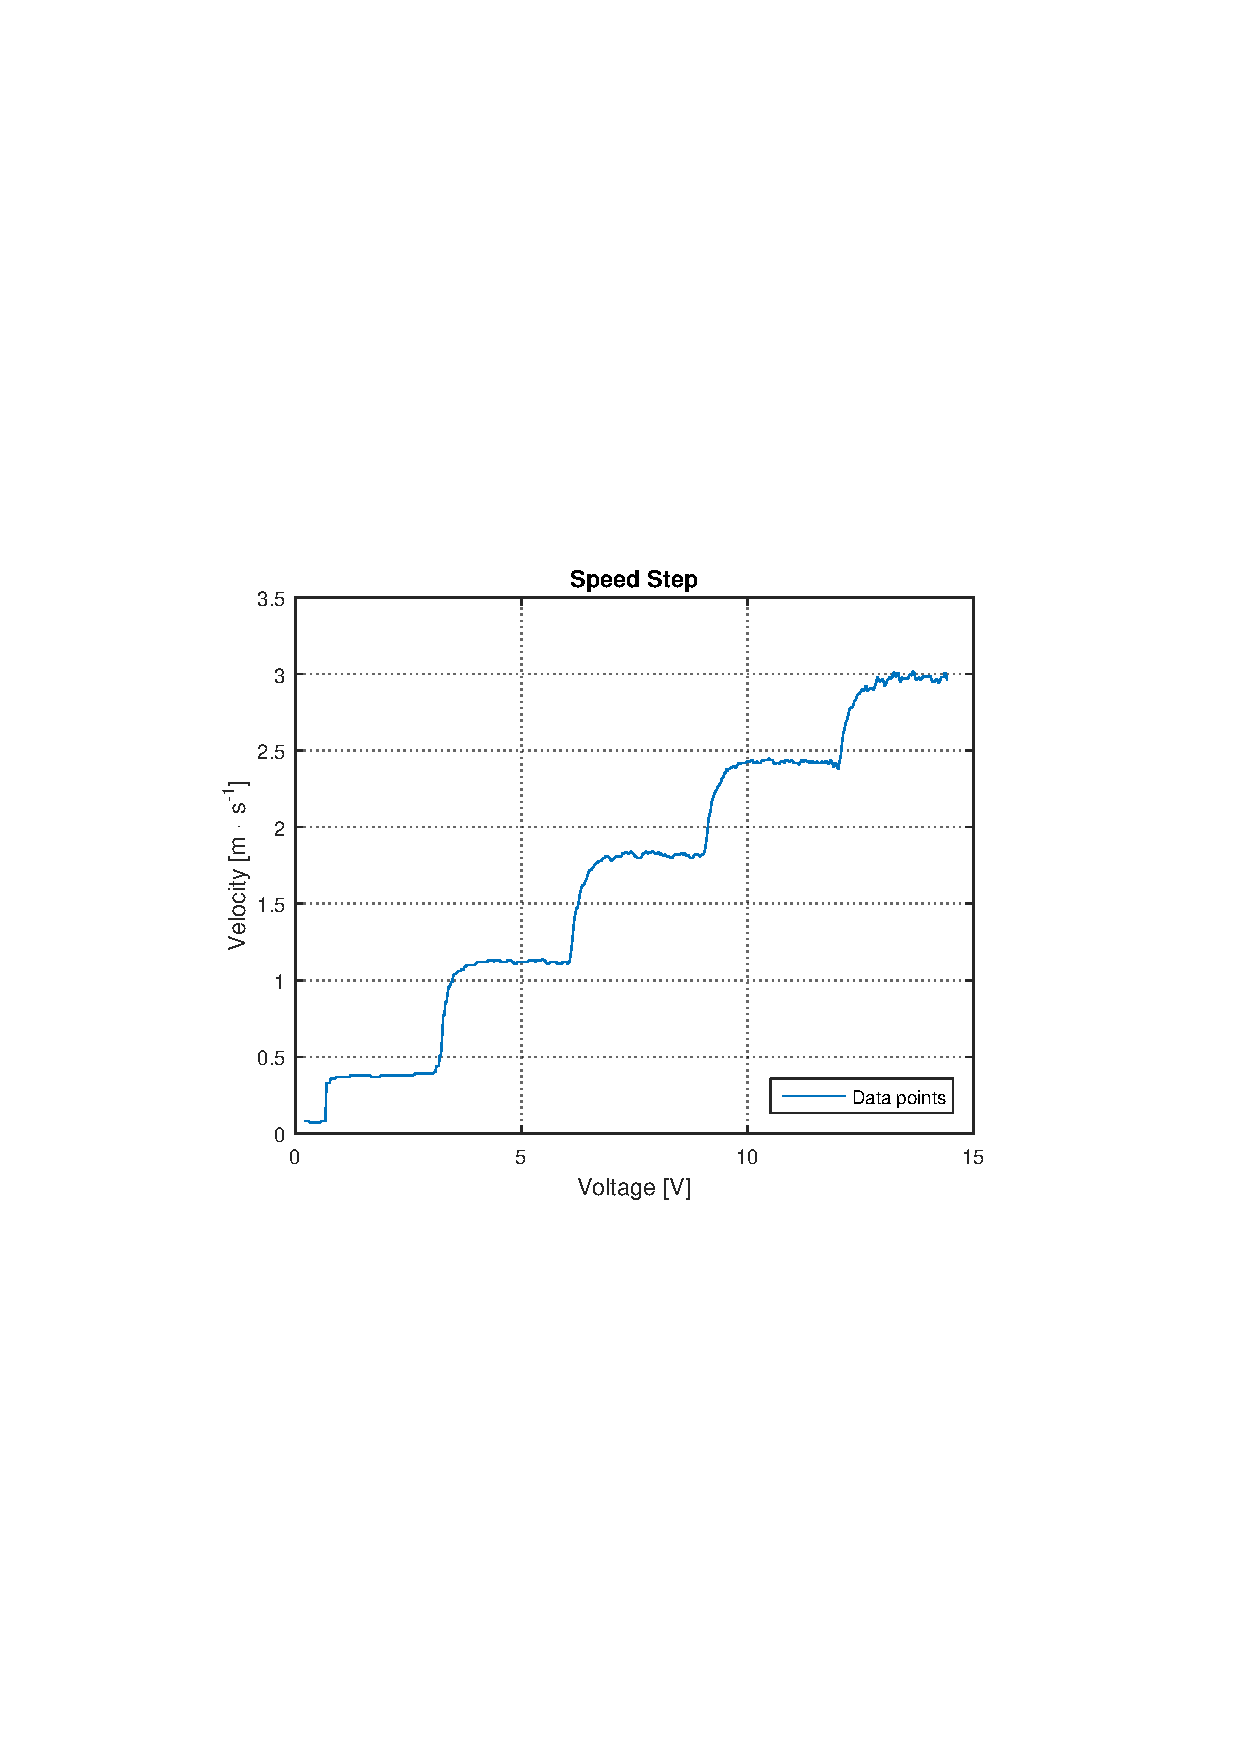
\includegraphics[width=1.4\textwidth]{figures/SpeedStep.pdf}
  }
  \caption{A plot of a measured armature resistance, with a red line indicating the an average value.}
  \label{SpeedStepGainTest}
\end{figure}\todo{fig text}

from \figref{SpeedStepGainTest} it is seen that for each two seconds the vehicle's velocity is increased by 20 percent. By taking the the average value of the vehicles steady state speed at each velocity, it is possible to get a gain of the vehicle, this is illustrated in \figref{GainOfEachSpeedStep}.

\begin{figure}[H]
  \centering
 	%Trim margins @:   left        bottom       right       top
 	\adjustbox{ trim = {.15\width} {.30\height} {.15\width} {.30\height}, clip }
  {
    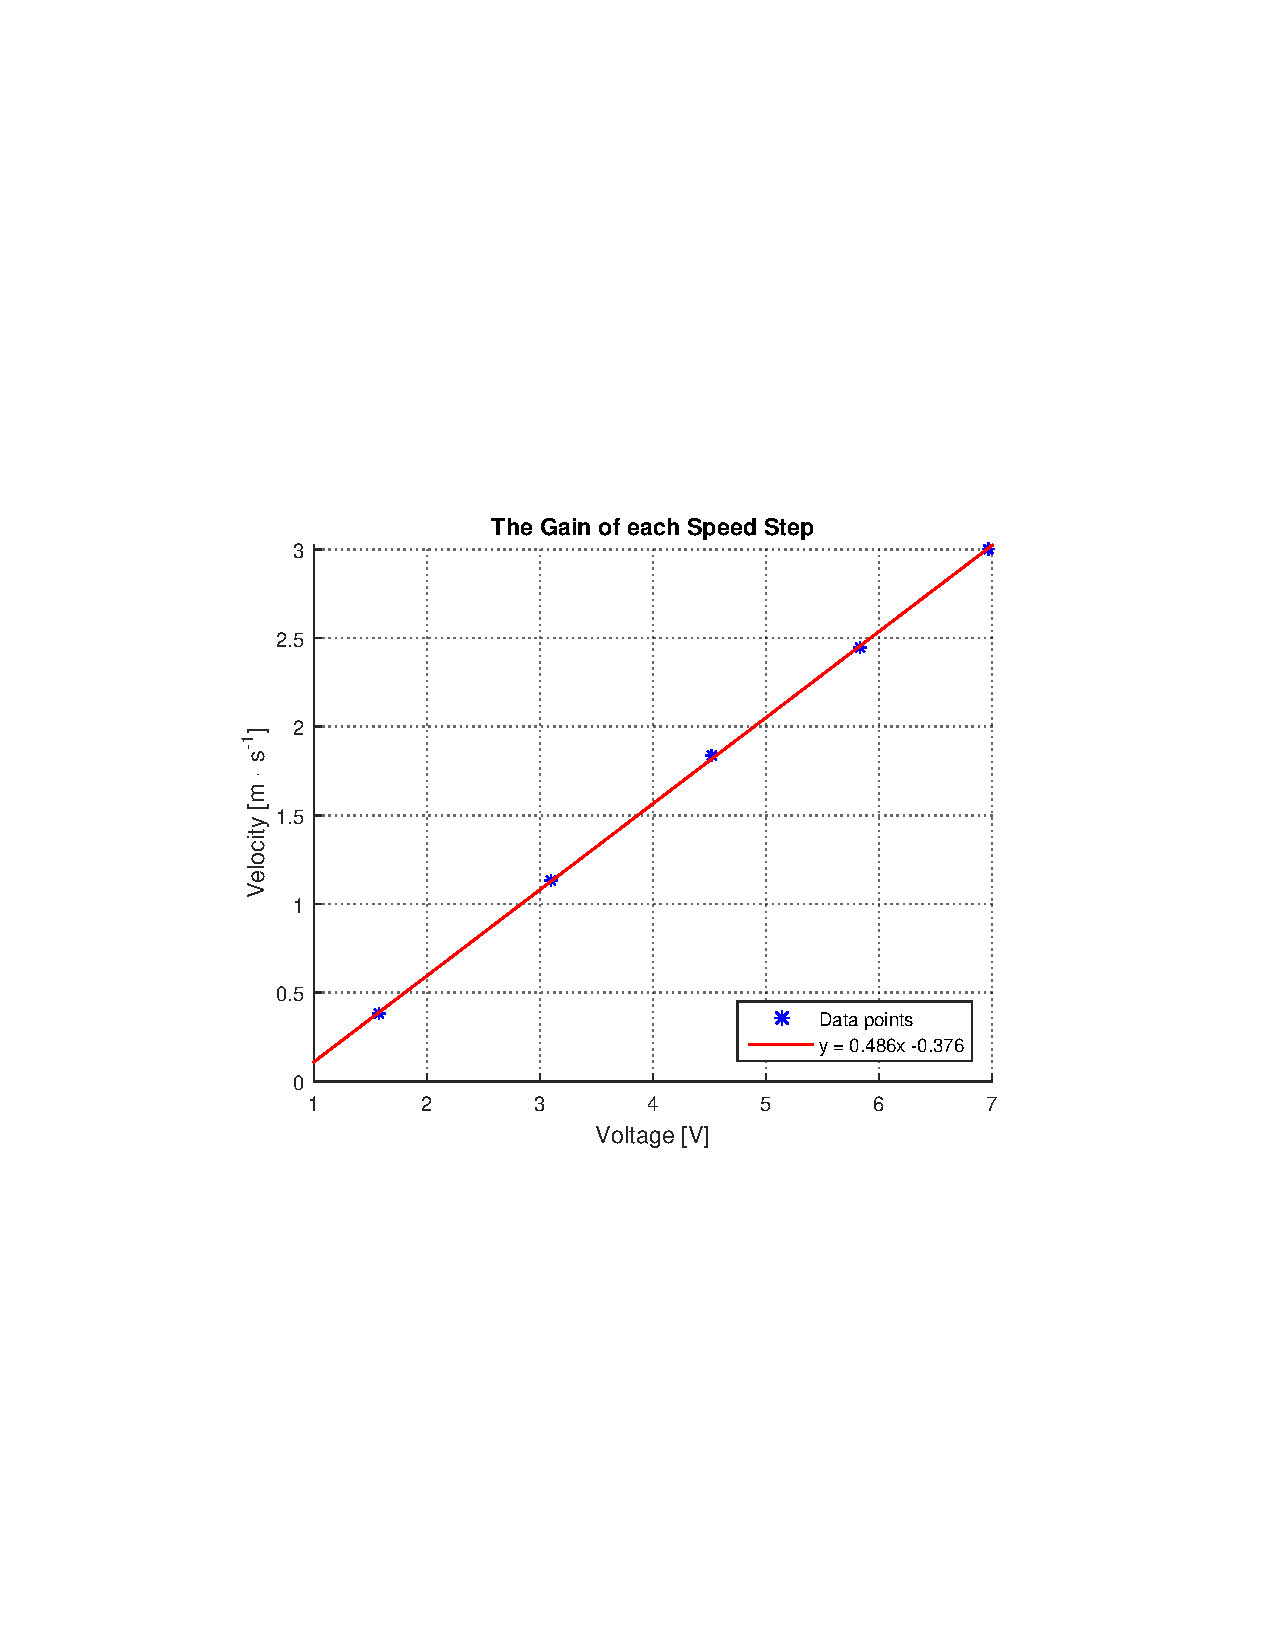
\includegraphics[width=1.4\textwidth]{figures/GainOfEachSpeedStep.pdf}
  }
  \caption{A plot of a measured armature resistance, with a red line indicating the an average value.}
  \label{GainOfEachSpeedStep}
\end{figure}\todo{fig text}

By making a least square line going through the average gain value at each velocity, it is possible to get the gain and the offset created by the stiction from the least square line. The equation for the least square line is seen on \figref{GainOfEachSpeedStep}. The Gain and the offset created by the stiction is therefore:

\begin{flalign}
\eq{K_G}{0,485} \ \si{m \cdot s^{-1} \cdot V^{-1}}&\\
\eq{\Delta v}{0,376} \ \si{m \cdot s^{-1}}&
\end{flalign}

